\documentclass[a5paper,12pt]{article}
\usepackage[utf8]{inputenc}
\usepackage[IL2]{fontenc}
\usepackage{listings}
\usepackage{amssymb}
\usepackage{amsmath}
\usepackage{enumitem}
\usepackage{url}
\usepackage{graphicx}
\usepackage[czech]{babel}
\usepackage[top=2cm, bottom=2cm, left=2cm, right=2cm, landscape]{geometry}
%\usepackage[landscape]{geometry}
\usepackage{amsthm}
\usepackage{paralist}
\usepackage{array}
\newtheorem*{thm}{Teor\'em}
\newtheorem*{mydef}{Defin\'icia}
\newtheorem*{exampl}{Pr\'iklad}
\title{Teorie her}
\author{Michal Abaffy, Marek Bryša, Jan Kovář}
\date{Brno, \today}
\begin{document}
  \maketitle
  \section{Úvod}
    Teorie her je matematická disciplína, která analyzuje široké spektrum konfliktních rozhodovacích situací, které mohou nastat kdekoliv, kde dochází ke střetu zájmů. Herně-teoretické modely se pak snaží tyto konfliktní situace nejen analyzovat, ale sestavením matematického modelu daného konfliktu a pomocí výpočtů se snaží nalézt co nejlepší strategie pro konkrétní účastníky takových konfliktů.

    \subsection{Reprezentace hry}
    Hra je charakterizována dvěma nebo více hráči, množinami akcí (tahů), které tito hráči mohou vykonat v určitých okamžicích, a možnými zisky, kterých hráči mohou dosáhnout. Zisk každého hráče nezávisí pouze na jím vykonaných akcích, ale také na akcích ostatních hráčů. Formálněji, existuje několik odlišných herních reprezentací: \emph{normální forma} (neboli \emph{strategická forma}), \emph{extenzivní forma} či \emph{kooperativní forma} (neboli \emph{forma charakteristické funkce}). Každé přináší jiný popis hry, a slouží tak k~různým účelům. Hra v~extenzivní formě může být využita ke specifikaci hry v~normální formě a hra v~normální formě může být použita k~definici hry v~kooperativní formě, nikoliv však naopak.

    \subsubsection{Klasifikace her}
    Rozlišujeme statické a dynamické hry. U~statických her vykonávají hráči své tahy současně, případně neznají zvolené tahy protihráčů. U~dynamických her hráči táhnou postupně, a mohou tedy reagovat na předchozí tahy protihráčů. Podle toho, zda každý z~hráčů zná zisky všech hráčů ve všech možných výsledcích hry, rozlišujeme hry s~úplnými a neúplnými informacemi.
       
    Na základě tohoto členění klasifikujeme hry do čtyř skupin:
    \begin{compactitem}
    \item statické hry s úplnými informacemi,
    \item dynamické hry s úplnými informacemi,
    \item statické hry s neúplnými informacemi,
    \item dynamické hry s neúplnými informacemi.
    \end{compactitem}

    U~her s~neúplnými informacemi pracujeme s~pravděpodobnostními rozděleními, kterými se řídí zisky protihráčů. Zde se budeme zabývat hrami s~úplnými informacemi.
     
    \subsubsection{Statické hry a normální forma}
    \emph{Strategie} hráče je kompletní plán akcí, který specifikuje, jaké tahy má hráč vykonat v~závislosti na dosavadním průběhu hry. V~případě statických her pojmy akce a strategie splývají. 

    Ke specifikaci statických her s~úplnými informacemi slouží normální forma.

    %\fbox{
    %\parbox{.8\textwidth}{
    \emph{Hra v normální formě} obsahuje následující prvky:
    \begin{compactitem}
    \item množinu hráčů: $\{1,\dots , n\}$,
    \item množinu strategií $S_i$ pro každého hráče $i \in \{1,\dots , n\}$,
    \item výplatní funkci $u_i : S_1 \times \dots \times S_n \rightarrow \mathbb{R}$ pro každého hráče $i \in \{1,\dots , n\}$.
    \end{compactitem}
    %}}

    Hra dvou hráčů v normální formě je nejčastěji charakterizována pomocí \emph{dvojmatice}.

    \begin{figure}[htb]
    \centering
    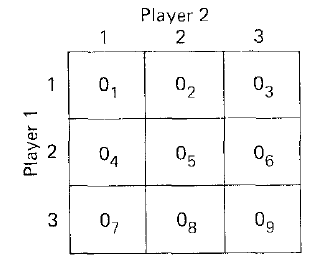
\includegraphics[scale=0.35]{1_3.png}
    \caption{Hra v normální formě v podobě dvojmatice \label{bimatrix}}
    \end{figure}

    Normální forma může být použita i~k~popisu dynamických her. Je však třeba specifikovat, kdy je který hráč na tahu, jaké akce může vykonat a jaké informace má o~dosavadním průběhu hry. Pojmy akce a strategie se u~dynamických her rozcházejí. Definujme nejprve extenzivní formu.

    \emph{Příklad:} Vězňovo dilema

    \subsubsection{Extenzivní forma}
    Extenzivní forma reprezentace hry specifikuje:
    \begin{compactitem}
    \item množinu hráčů,
    \item kdy je který hráč na tahu,
    \item jaké má hráč informace o dosavadním průběhu hry ve chvíli, kdy je hráč na tahu,
    \item množinu akcí, které může hráč podstoupit,
    \item výplatní funkci každého hráče jakožto funkci akcí podstoupených všemi hráči. 
    \end{compactitem}

    Jako první popsali hru pomocí extenzivní formy von Neumann a Morgenstern (1944) a poté Kuhn (1953). V~obou případech se jednalo o~konečné hry, tj. hry, ve kterých je konečný počet hráčů, tahů i akcí. Příkladem takových her jsou např. šachy nebo poker. Nicméně málokteré situace v ekonomice či politice jsou modelovány konečnými hrami. 

    Hra v extenzivní formě je nejčastěji zobrazována pomocí stromu. Jednoduchý trh v~prostředí duopolu je ilustrován Kuhnovým herním stromem. Jedná se o zjednodušený případ, kdy si každá ze dvou firem musí vybrat jednu ze tří možných úrovní produkce. Firmy se rozhodují současně. Jejich úrovně produkce určují tržní výstup a zisky obou firem. Na obrázku \ref{Kuhn} je popis této hry v extenzivní formě. Každý uzel reprezentuje stav, ve kterém se hra může nacházet (z~pohledu nezávislého pozorovatele). Hra začíná v~kořeni stromu (označeným $R$). Každý uzel, který není listem, je označen $P_i$, což indikuje, že je na tahu hráč $i$ a má na výběr z~tahů odpovídajícím větvím stromu vycházejícím z~tohoto uzlu. Listy stromu jsou označeny $O_j$ a reprezentují všechny možné výsledky hry. Každá cesta z~kořene do listu určuje možný průběh hry.

    \begin{figure}[htb]
    \centering
    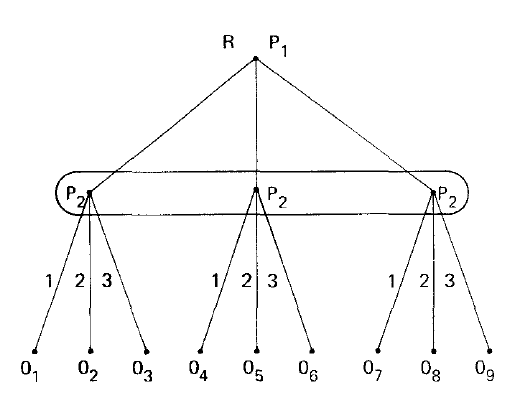
\includegraphics[scale=0.35]{1_1.png}
    \caption{Kuhnův herní strom \label{Kuhn}}
    \end{figure}

    V~mnoha situacích můžeme vyžadovat, aby hráči táhli současně (statické hry). Nezajímá nás, zda hráči táhli přesně ve stejném okamžiku, podstatné je to, že hráči v~okamžiku rozhodnutí o~svém tahu nemají informace o~tahu protihráčů. Nezáleží na tom, kdo táhne první, protože ostatní nejsou informováni. Tuto situaci znázorňujeme ve stromě tak, že propojíme (oválem či čárkovanou čarou) všechny uzly, o~nichž hráč neví, ve kterém z~nich se nachází. Tyto uzly tvoří tzv. \emph{informační množinu}. Ze všech uzlů jedné informační množiny musí vycházet stejné hrany. Extenzivní forma tedy umožňuje reprezentovat i statické hry. Obrázky \ref{bimatrix} a \ref{Kuhn} reprezentují tutéž hru v~normální a v~extenzivní formě.

    V~některých případech je třeba do hry zahrnout exogenní nejistotu. V~takové situaci přidáme do hry dalšího hráče $P_0$, nazývaného \emph{Příroda}. Kdykoliv je tento hráč na tahu, s~danými pravděpodobnostmi vybere jednu z větví. Příklad hry obsahující \emph{Přírodu} je na obrázku \ref{nature}.

    \begin{figure}[htb]
    \centering
    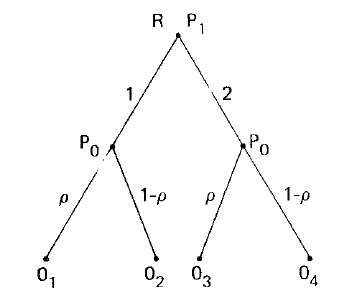
\includegraphics[scale=0.35]{1_2.png}
    \caption{ Hra obsahující hráče \emph{Příroda} \label{nature}}
    \end{figure}

    Hry, které obsahují pouze jednoprvkové informační množiny se nazývají hry s~\emph{perfektními informacemi}. Takovou hrou jsou šachy. V~každém okamžiku hry znají všichni hráči všechny detaily cesty z~kořene do současného uzlu. To neplatí pro poker, či pro aukce s~uzavřenými nabídkami.

    V~terminologii stromů a informačních množin můžeme \emph{strategii} definovat jako funkci, která každé informační množině hráče přiřadí jednu z~alternativ (tj. hran) vycházejících z~této informační množiny. 

    \subsubsection{Dynamické hry a normální (strategická) forma}
    Dynamické hry je možné také reprezentovat v~normální formě. Nyní ovšem rozlišujeme pojmy akce a strategie. V~záhlavích tabulky (resp. dvojmatice) nyní již nebudou akce, ale kombinace akcí, přesněji strategie.

    Uvažujme modifikaci hry v~extenzivní formě na obrázku~\ref{Kuhn}. Nahraďme informační množinu hráče $P_2$ dvěma informačními množinami, a to tak, že pokud hráč $P_1$ zvolí možnost 1, $P_2$ je informován, zvolí-li $P_1$ možnost 2 nebo 3, $P_2$ neví, ve kterém z~těchto dvou uzlů se nachází. Tato hra je v~normální formě reprezentována maticí $3 \times 9$, protože existuje 9 různých strategií pro $P_2$. Strategiemi hráče $P_2$ jsou uspořádané dvojice $(i,j)$, $i,j \in \{1,2,3\}$, které chápeme: \uv{jestliže $P_1$ hrál 1, hraj $i$, jinak hraj $j$}. 

    \subsubsection{Kooperativní (koaliční) forma}
    V~normální formě je kladen důraz na jedince, a to v~tom smyslu, že zisk hráče závisí na jím zvolené strategii a na strategiích zvolených ostatními hráči. Není přikládán význam možnostem spolupráce mezi hráči. Při studiu tvorby kartelů, mezinárodního obchodu, vyjednávání nebo jiných skupinových jevů může být kladen důraz na možné zisky ze spolupráce mezi jednotlivými účastníky. 

    Uvažujme následující hru dvou hráčů v normální formě (jedná se o obecné vězňovo dilema), $a_i > b_i > c_i > d_i$.

    \begin{figure}[htb]
    \centering
    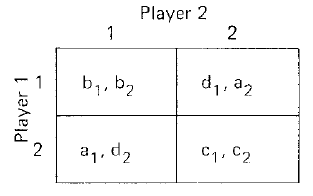
\includegraphics[scale=0.35]{1_4.png}
    \caption{ Obecné vězňovo dilema v~normální formě \label{prisoner}}
    \end{figure}

    %Můžeme rozlišit dvě různé formy této hry, a to v~závislosti na tom, zda přijmeme předpoklad o~přenositelnosti užitku.

    Označme $\upsilon(S)$ zisk, kterého může dohromady dosáhnout koalice hráčů $S$, pokud hrají jako jeden hráč. $\upsilon$ nazýváme \emph{charakteristická funkce}. Je to funkce z~podmnožin všech hráčů do reálných čísel. Pro hru $n$ hráčů existuje $2^n-1$ neprázdných koalic.

    Označení $\upsilon(\overline{ij})$ je použito ke specifikaci konkrétní koalice sestávající z~hráčů $i$ a $j$. Charakteristická funkce pro vězňovo dilema na obrázku~\ref{prisoner} je následující:
    \begin{gather*}
    \upsilon(\emptyset)=0, \quad \upsilon(\overline{1})=c_1, \quad \upsilon(\overline{2})=c_2\\
    \upsilon(\overline{12})=\max \{ (b_1+b_2),(a_1+d_2),(a_2+d_1), \}.
    \end{gather*}

    Charakteristická funkce může být považována za počáteční řešení hry v~tom smyslu, že její výpočet poskytne náhled do struktury hry. V~tomto příkladě byly hodnoty spočteny jako odpovědi na otázku, jakého maximálního zisku může koalice dosáhnout za předpokladu, že ostatní hráči se snaží tento zisk minimalizovat. Nejlepší, co může udělat sám hráč $P_1$, resp. $P_2$, je hrát druhou strategii a získat $c_1$, resp. $c_2$. Dohromady mohou hráči získat $b_1+b_2$. V~tomto příkladě je oprávněné vyhodnotit $\upsilon(\overline{1})$ jako $c_1$, protože hráč $P_2$ tím, že minimalizuje zisk hráče $P_1$, současně optimalizuje své vlastní skóre. To nemusí být pravda obecně, jako protipříklad slouží následující hra.

    \begin{figure}[htb]
    \centering
    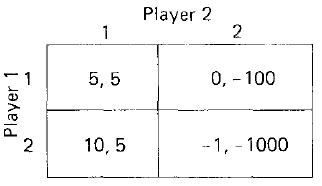
\includegraphics[scale=0.35]{1_5.png}
    \caption{}
    \end{figure}
     
     Zde charakteristická funkce nabývá hodnot
    \[
    \upsilon(\emptyset)=0, \quad \upsilon(\overline{1})=0, \quad \upsilon(\overline{2})=5, \quad
    \upsilon(\overline{12})=15.
    \]

    Zde je poněkud nelogické považovat pozici  hráče $P_2$ za nejvýhodnější. Paradox je v~zacházení s~hrozbami. Výpočet charakteristické funkce pro hráče $P_1$ nebere v~úvahu vysoké náklady hráče $P_2$ spojené s~výběrem strategie 2.

    Můžeme definovat \emph{zobecněnou charakteristickou funkci} (či \emph{charakterizující funkci}) $V(S)$, která pro každou množinu hráčů $S$ určuje množinu optimálních dosažitelných zisků.

    Způsob definice zobecněné charakteristické funkce je ilustrován na obrázku \ref{charfce}, který zobrazuje příklad se třemi hráči. Osy $\alpha_1,\alpha_2,\alpha_3$ znázorňují zisky obdržené po řadě hráči 1, 2 a 3. Zacházíme s $V(S)$, jako by to byl válec, který vyřízne část Paretovsky optimální plochy pro hru $n$ hráčů jako celek. Například koalice $\overline{12}$ může získat alespoň tolik, kolik se jí dostává v~libovolném bodě části Paretovsky optimální množiny $ABC$ ohraničené $EFC$.

    \begin{figure}[h!tb]
    \centering
    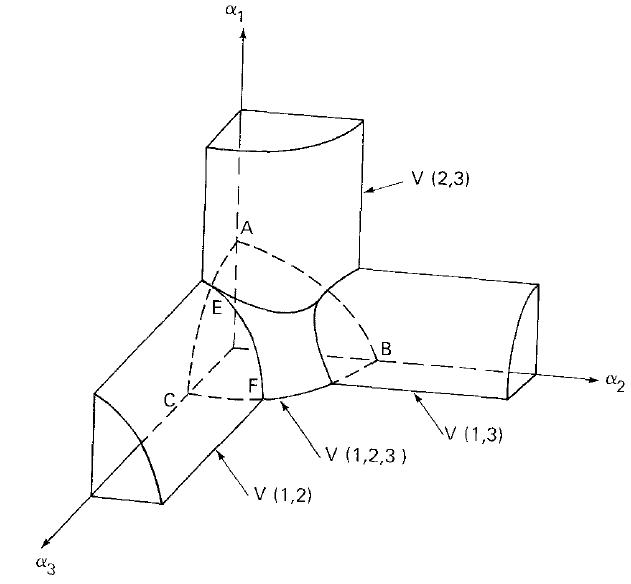
\includegraphics[scale=0.35]{1_6.png}
    \caption{Zobecněná charakteristická funkce \label{charfce}}
    \end{figure}
\clearpage    
  \section{Řešení}
    \subsection{Hry v strategickej forme}
      \v{C}as\v{t} 1: Ka\v{z}d\'y s\'am za seba

      \begin{mydef}
      Nech $X$ je mno\v{z}ina strat\'egii $i$-teho hr\'a\v{c}a a $Z$ je mno\v{z}ina strat\'egii ostatn\'ych hr\'a\v{c}ov. Nech $u_{i}: X \times Z \to \mathbb{R}$ je \'u\v{z}itkov\'a funkcia $i$-teho hr\'a\v{c}a. Strat\'egia $x \in X$ {\bf dominuje} strat\'egii $y \in X$ ak pre v\v{s}etky mo\v{z}n\'e strat\'egie $z \in Z$ plat\'i $u_{i}(x,z) \geq u_{i}(y,z)$ a existuje strat\'egia $z' \in Z$ tak\'a, \v{z}e $u_{i}(x,z') > u_{i}(y,z')$.

      \end{mydef}

      \begin{mydef}
      Strat\'egia $x\in X$ sa naz\'yva {\bf nedominovan\'a}, ak neexistuje strat\'egia $x' \in X$, ktor\'a by jej dominovala.
      \end{mydef}

      V hr\'ach, kde ka\v{z}d\'y hr\'a s\'am za seba nem\'a zmysel hra\v{t} dominovan\'e strat\'egie.
            
      \begin{mydef}
      Nech $X$ je mno\v{z}ina strat\'egii hr\'a\v{c}ov, nech $u_{i}$ je \'u\v{z}itkov\'a funkcia $i$-teho hr\'a\v{c}a. Situ\'acia $x \in X$ {\bf dominuje pod\v{l}a Pareta} situ\'acii $x' \in X$, ak \[\forall i: u_{i}(x) \geq u_{i}(x') \textrm{ a } \exists i: u_{i}(x) > u_{i}(x')\]

      \end{mydef}

      \begin{mydef}
      Situ\'acia $x\in X$ sa naz\'yva {\bf optim\'alna pod\v{l}a Pareta}, ak neexistuje situ\'acia, ktor\'a by jej dominovala pod\v{l}a Pareta. 
      \end{mydef}

      Niektor\'e situ\'acie optim\'alne pod\v{l}a Pareta mo\v{z}u prinies\v{t} niektor\'emu z hr\'a\v{c}ov menej, ako si s\'am dok\'a\v{z}e zaru\v{c}i\v{t}. Vi\v{d} pr\'iklad neskor. 

      Mo\v{z}nost zavies\v{t} \emph{imputation set}, kde s\'u tie situ\'acie, ktor\'e s\'u optim\'alne pod\v{l}a Pareta a ka\v{z}d\'y hr\'a\v{c} dostane aspo\v{n} to\v{l}ko, ko\v{l}ko si vie s\'am garantova\v{t}.
      
      \begin{mydef}
      Nech $X_{i}$ je mno\v{z}ina strat\'egii $i$-teho hr\'a\v{c}a a $Z_{i}$ je mno\v{z}ina strat\'egii ostatn\'ych hr\'a\v{c}ov. Nech $u_{i}: X_{i} \times Z_{i} \to \mathbb{R}$ je \'u\v{z}itkov\'a funkcia $i$-teho hr\'a\v{c}a. Situ\'acia $x=(y,z), y\in X_{i}, z\in Z_{i}$ sa naz\'yva {\bf rovnov\'a\v{z}na pod\v{l}a Nasha}, ak plat\'i
      \[\forall i, \forall y' \in X_{i}: u_{i}(x) \geq u_{i}(y',z)\]
      \end{mydef}

      Pretlmo\v{c}en\'e: Situ\'acia je rovnov\'a\v{z}na pod\v{l}a Nasha, ak si \v{z}iaden z hr\'a\v{c}ov s\'am nepomo\v{z}e k lep\v{s}ej v\'yhre. V [5], Nash dok\'azal nasleduj\'uci teor\'em.

      \begin{thm}
      Existuj\'u hry, kde pri \v{c}ist\'ych strat\'egi\'ach neexistuje situ\'acia RPN, av\v{s}ak pri zmie\v{s}an\'ych strat\'egi\'ach m\'a ka\v{z}d\'a hra situ\'aciu RPN.
      \end{thm}
      
      \begin{exampl} Uva\v{z}ujme nasleduj\'uce dve hry dvoch hr\'a\v{c}ov v strategickej forme:

      \

      \begin{tabular}{ l l l l}
      Strat\'egie            & 1 & 2 & 3 \\
      \hline
       1  & (1,6) & (0,2) & (1,3) \\
       2  & (2,3) & (2,2) & (2,3) \\
      \end{tabular}

      \

      \

      \begin{tabular}{l l l}
      Strat\'egie            & 1 & 2 \\
      \hline
       1  & (6,6) & (2,0) \\
       2  & (0,2) & (5,5) \\
      \end{tabular}

      \

      Pre obe hry. N\'ajdite nedominovan\'e strat\'egie pre oboch hr\'a\v{c}ov, n\'ajdite v\v{s}etky situ\'acie optim\'alne pod\v{l}a Pareta a rovnov\'a\v{z}ne pod\v{l}a Nasha a imputation sety.

      \end{exampl}
    \subsection{Koali\v{c}n\'e hry}
      \v{C}as\v{t} 2: Koali\v{c}n\'e hry

      Predpoklady:

      - M\'ame mno\v{z}inu hr\'a\v{c}ov $N$. Majme \v{l}ubovoln\'u koal\'iciu $S \subseteq N$. Uva\v{z}ujme, \v{z}e hr\'a\v{c}i z $S$ navz\'ajom spolupracuj\'u. Mo\v{z}u zvoli\v{t} spolo\v{c}n\'u strat\'egiu, ktor\'a im garantuje ist\'u sumu $v(S)$, o ktor\'u sa n\'asledne mo\v{z}u ist\'ym sposobom rozdeli\v{t}. 

      - Technick\'y detail: v\'yhry musia by\v{t} v spolo\v{c}nej mene (alebo aspo\v{n} prevediteln\'e do spolo\v{c}nej meny), a ka\v{z}d\'y hr\'a\v{c} si ka\v{z}d\'u v\'yhru cen\'i rovnako (\'u\v{z}itkov\'e funkcie roznych hr\'a\v{c}ov su rovnak\'e).

      - Zjavne: $S \cap T = \emptyset \implies v(S \cup T) \geq v(S) + v(T)$.

      - Po\v{z}adujeme: $v(\emptyset)=0$.

      \

      Aj in\'y typ koali\v{c}n\'ych hier: hr\'a\v{c}i mo\v{z}u spolupracova\v{t} v \v{l}ubovolnej koal\'icii, ale v\'yhry nie s\'u prenosn\'e. S tak\'ymto typom hier sa pracuje zlo\v{z}itej\v{s}ie, my sa nimi nebudeme zaobera\v{t}.
      
    \subsection{Jadro (The core)}
      Chcen\'e rie\v{s}enie probl\'emu (nemus\'i existova\v{t}): pre ka\v{z}d\'u koal\'iciu plat\'i, \v{z}e s\'u\v{c}et v\'yhier jej hr\'a\v{c}ov je aspo\v{n} to\v{l}ko, ko\v{l}ko garantuje \'u\v{c}as\v{t} v koal\'icii. Form\'alne:

      Rie\v{s}enie je {\bf payoff vector} $(x_{1}, ..., x_{n})$, kde $x_{i}$ predstavuje v\'yhru $i$-teho hr\'a\v{c}a a plat\'i $\sum_{i=1}^{n} x_{i} = v(N)$.

      \begin{mydef}
      Jadro s\'u tak\'e payoff vectory, kde plat\'i:
      \[\forall S \subseteq N: \sum_{i \in S}x_{i} \geq v(S)\]
      \end{mydef}
      \begin{exampl} Nie v\v{z}dy mus\'i tak\'eto rie\v{s}enie existova\v{t}. 

      $v(\emptyset)=0,$

      $ v(\{1\})=v(\{2\})=v(\{3\})=0,$

      $v(\{1,2\})=v(\{1,3\})=v(\{2,3\})=1, $

      $v(\{1,2,3\})=1$.

      \end{exampl}

      V jednoduch\'ych pr\'ipadoch rie\v{s}ime tak, \v{z}e zvol\'ime koal\'iciu v\v{s}etk\'ych hr\'a\v{c}ov a nakreslen\'im.

      \begin{exampl}
      $v(\emptyset)= v(\{1\})=v(\{2\})=v(\{3\})=0,$

      $v(\{1,2\})= 1, v(\{1,3\})=2, v(\{2,3\})=3$

      $v(\{1,2,3\})= 4$

      \end{exampl}

      Rie\v{s}enie: nakresl\'ime trojuholn\'ik $(4,0,0), (0,4,0), (0,0,4)$ a vkres\v{l}ujeme do\v{n} nerovnosti.

      V pr\'ipade, \v{z}e jadro neexistuje, mo\v{z}eme chcie\v{t} od rie\v{s}enia aspo\v{n}, aby to bol takzvan\'y {\bf rozumn\'y payoff vector}, teda by malo sp\'l\v{n}a\v{t}: 
      \[ \forall i: x_{i} \leq \max_{S}\{v(S)-v(S-\{i\})\}\]


      V\'yhody: 

      - Satisfy all subgroup rationality, i.e., no subgroup is offered less than it could obtain by itself.

      \

      Nev\'yhody: 

      - Jadro nemus\'i existova\v{t}.

      - Mo\v{z}e n\'ajs\v{t} mno\v{z}inu rie\v{s}en\'i a nie je jasn\'e, ktor\'y hr\'a\v{c} ko\v{l}ko dostane.

      \

      Daj\'u sa \v{c}iasto\v{c}ne odstr\'ani\v{t} (no vznikn\'u nov\'e nedostatky) zaveden\'im siln\'eho (slab\'eho) $\epsilon$-core, kde rie\v{s}enie $x$ mus\'i sp\'l\v{n}a\v{t}:
      \[\forall S \subseteq N: \sum_{i \in S}x_{i} \geq v(S) - \epsilon  \textrm{, respekt\'ive }\] 
      \[\forall S \subseteq N: \sum_{i \in S}x_{i} \geq v(S) - |S|\epsilon \]

    \subsection{Simple games}
      Simple games sp\'l\v{n}aj\'u nasleduj\'uce axi\'omy:

      (1) $\forall S \subseteq N: v(S)=0$ or $v(S)=1$.

      (2) $v(\emptyset)=0$

      (3) $v(N)=1$

      (4) No losing set contains a winning subset. (Pod\v{l}a m\v{n}a zbyto\v{c}n\'y, plynie z axi\'omov pre charakteristick\'u funkciu $v$.)

      \

      V\'yznamn\'a podtrieda simple games ({\bf rozhoduj\'uce SG}) sp\'l\v{n}a i nasledovn\'y axi\'om:

      (5)  $\forall S \subseteq N: v(S) + v(N - S)= 1$.

    \subsection{Shapley vector}
      Jednoduch\'e hry va\v{c}\v{s}inou nemaj\'u rie\v{s}enie v podobe jadra.

      Rie\v{s}enie (nielen pre RSG): {\bf Shapleyho vector $x$}
      \[x_{i}(v)=\sum_{S \subseteq N}\frac{(n-s)!(s-1)!}{n!}(v(S)-v(S-\{i\}))\]

      Predpoklady ved\'uce k Shapleyho vectoru: aditivita na nez\'avisl\'ych hr\'ach; symetria hr\'a\v{c}ov; linearita pri n\'asoben\'i skal\'arom (hra a vektor); $\sum_{i \in S} x_{i}(u) = u(S)$, kde $S \subseteq N$ je \v{l}ubovoln\'a koal\'icia, ktor\'a obsahuje v\v{s}etk\'ych podstatn\'ych hr\'a\v{c}ov (hr\'a\v{c} $i$ je podstatn\'y, ak existuje koal\'icia $S$, t\v{z} $v(S \cup \{i\})> v(S) + v(\{i\})$).

      \

      Interpret\'acia: Each individual is assumed to enter every possible coalition in every way randomly, and he is then assigned the expected value of the incremental gain he brings to all.

      \begin{exampl}
      Vo\v{l}by do parlamentu. Zvolen\'ych 5 str\'an a nech $A,B,C,D,E$ zna\v{c}ia po\v{c}et poslancov jednotliv\'ych str\'an. $A=55, B=30, C=25, D=22, E=18$. V\'i\v{t}azn\'e koal\'icie s\'u tie, ktor\'e maj\'u viac ako 75 poslancov. Spo\v{c}\'itajte SV.
      \end{exampl}

      \emph{Rie\v{s}enie:} V\'i\v{t}azne koal\'icie (s \v{c}iarkou s\'u zna\v{c}en\'i t\'i, ktor\'ych pr\'ichod do koal\'icie zmen\'i nev\'i\v{t}azn\'u koal\'iciu na v\'i\v{t}zn\'u): $A'B', A'C', A'D', A'BC, A'BD, A'B'E, A'CD, A'C'E, A'D'E, B'C'D', ABCD,$ $ A'BCE, A'BDE, A'CDE, B'C'D'E, ABCDE$.

      $x_{A} = 3 \frac{3!1!}{5!} + 6 \frac{2!2!}{5!} + 3 \frac{1!3!}{5!}= \frac{18+24+18}{120}=\frac{1}{2}$

      $x_{B} = 1 \frac{3!1!}{5!} + 2 \frac{2!2!}{5!} + 1 \frac{1!3!}{5!}= \frac{6+8+6}{120} = \frac{1}{6}$

      $x_{C} = 1 \frac{3!1!}{5!} + 2 \frac{2!2!}{5!} + 1 \frac{1!3!}{5!}= \frac{6+8+6}{120} = \frac{1}{6}$

      $x_{D} = 1 \frac{3!1!}{5!} + 2 \frac{2!2!}{5!} + 1 \frac{1!3!}{5!}= \frac{6+8+6}{120} = \frac{1}{6}$

      $x_{E} = 0$

      Kontrola: $x_{A}+x_{B}+x_{C}+x_{D}+x_{E}=1=v(N)$.
      
    \subsection{Stable set}
      Predpoklad: plne kooperat\'ivna hra, zvol\'i sa ve\v{l}k\'a koal\'icia a jej zisk sa distribuuje pomocou payoff vectoru medzi hr\'a\v{c}ov.
       
      \begin{mydef}
      {\bf Imputation} je tak\'y payoff vector $x$, kde \v{z}iaden hr\'a\v{c} nedostane menej ako si dok\'aze s\'am zaru\v{c}i\v{t}. 
      \[ \forall i:x_{i} \geq v(\{i\})\]
      \end{mydef}


      \begin{mydef}
      Majme hru $(N,v)$ a nech $x,y$ s\'u dve imputations $(N,v)$. {\bf $x$ dominuje $y$}, ak $\exists S \neq \emptyset$, t\v{z} $\forall i \in S :x_{i} > y_{i}$ a $\sum_{i \in S} x_{i} \leq v(S)$ (Pre\v{c}o nie rad\v{s}ej  $\sum_{i \in S} y_{i} < v(S)$? ).	
      \end{mydef}

      In other words, players in $S$ prefer the payoffs from $x$ to those from $y$, and they can threaten to leave the grand coalition if $y$ is used because the payoff they obtain on their own is at least as large as the allocation they receive under $x$. 

      \begin{mydef}
      A {\bf stable set} is a set of imputations that satisfies two properties:

      Internal stability: No payoff vector in the stable set is dominated by another vector in the set.

      External stability: All payoff vectors outside the set are dominated by at least one vector in the set.
      \end{mydef}

      Von Neumann povodne myslel, \v{z}e ka\v{z}d\'a plne kooperat\'ivna koali\v{c}n\'a hra m\'a stable set rie\v{s}enie. Nie je tomu tak.
      
    \subsection{Jadro (The kernel)}
      \begin{mydef}
      Majme hru $(N,v)$ a payoff vector $x$.
      \[s_{ij}^{v}(x):=\max_{S \subseteq N-\{j\}; i \in S}\{v(S) - \sum_{k \in S}x_{k}\}\]
      \end{mydef}

      \v{C}o $s_{ij}^{v}(x)$ predstavuje? 

      Predpokladajme, ze $j$ chce vyst\'upi\v{t} z ve\v{l}kej koal\'icie, kde sa prerozde\v{l}uje pod payoff vectorom $x$. Predpokladajme, \v{z}e ostatn\'i hr\'a\v{c}i s\'u spokojn\'i so svojou \v{c}as\v{t}ou $x_{k}$. Tak\v{z}e ak $j$ sa rozhodne nespolupracova\v{t}, hr\'a\v{c} $i$ mo\v{z}e z\'iska\v{t} maxim\'alne $s_{ij}^{v}(x)$, ak ostatn\'i hr\'a\v{c}i bud\'u s\'uhlasi\v{t} s vytvoren\'im koal\'icie S, kde ich zisk zo zisku koal\'icie bude rovn\'y ich zisku v povodnom payoff vectore. 

      Intuit\'ivne, ak $s_{ij}^{v}(x) > s_{ji}^{v}(x)$, $i$ m\'a va\v{c}\v{s}iu vyjedn\'avaciu silu ako $j$ pri payoff vectore $x$.

      Od dobr\'eho rie\v{s}enia o\v{c}ak\'avame, \v{z}e ka\v{z}d\'a dvojica hr\'a\v{c}ov bude ma\v{t} vo\v{c}i sebe rovnak\'u vyjedn\'avaciu silu. Plat\'i ale, \v{z}e hr\'a\v{c} $i$ je odoln\'y vo\v{c}i hrozb\'am in\'ych hr\'a\v{c}ov, ak $x_{i}-v(\{i\})=0$, preto\v{z}e mo\v{z}e zdrhn\'u\v{t} a spravi\'t si vlastn\'u koal\'iciu.

      \begin{mydef}
      Jadro hry obsahuje tak\'e imputations, kde \v{z}iadny hr\'a\v{c} nem\'a nad \v{z}iadnym hr\'a\v{c}om vyjedn\'avaciu silu, 
      \[ [s_{ij}^{v}(x) - s_{ji}^{v}(x)][x_{j}-v(\{j\})] \leq 0 \textrm{ and}\]
      \[ [s_{ji}^{v}(x) - s_{ij}^{v}(x)][x_{i}-v(\{i\})] \leq 0 \]

      \end{mydef}

      Plat\'i nasleduj\'uca veta [4]:

      \begin{thm}
      Ka\v{z}d\'a koali\v{c}n\'a hra m\'a nepr\'azdny kernel. 
      \end{thm}

\clearpage
  \section{Aplikace v ekonomických experimentech}
    \subsection{Hra diktátor}
      \emph{Diktátor} je nejjednodušší možná hra nebo spíše situace individuálního rozhodnutí,
      která může osvětlit preference ohledu na druhé. Tato hra má dva hráče: navrhovatele a příjemce.
      Navrhovatel rozhodne, jak se má rozdělit obdaření dané velikosti mezi něho a příjemce,
      což se pak také stane. Role příjemce je čistě pasivní.

      Implementace v laboratoři může vypadat takto: obdaření \$10 je poskytnuto experimentátorem jako
      \uv{dar z nebes}. Testované subjekty jsou náhodně náhodně rozděleny mezi navrhovatele a příjemce.
      Anonymita rozhodnutí a párování je zaručena.
        
      Tento experiment byl poprvé uveden v Forsythe et al. (1994) s těmito výsledky:
      \begin{compactitem}
        \item
          Je zjevné, že mnoho subjektů se nechová zcela sobecky, což odporuje konvenční teorii založené na
          ohledech na sebe.
        \item
          Tento výsledek byl od té doby mnohokrát ověřen. Typicky více než 60\% subjektů předá kladnou částku,
          průměrné 20\% obdaření. Toto je však velmi závislé na procedurálních detailech, viz dále.
      \end{compactitem}
      Cherry et al. (2002) říka, že pokud je obdaření nutno \uv{vydělat} např. tak, že navrhovately se stali ti,
      kteří uspěli ve vědomostním kvízu, převod kladných částek prakticky vymizí. (zde byla anonymita zaručena i
      vůči experimetátorovi)
      
      List (2007) ukazuje, že pokud je navrhovateli navíc dána možnost vzít peníze příjemci, prevod kladných částek
      opět zmizí a nejčastějším návrhem se stane sebrání co nejvíc peněz od příjemce. Pokud dále je obdaření vyděláno,
      přibližne 70\% navrhovatelů neprovode žádný převod, zbytek opět sebere, co může.\\
      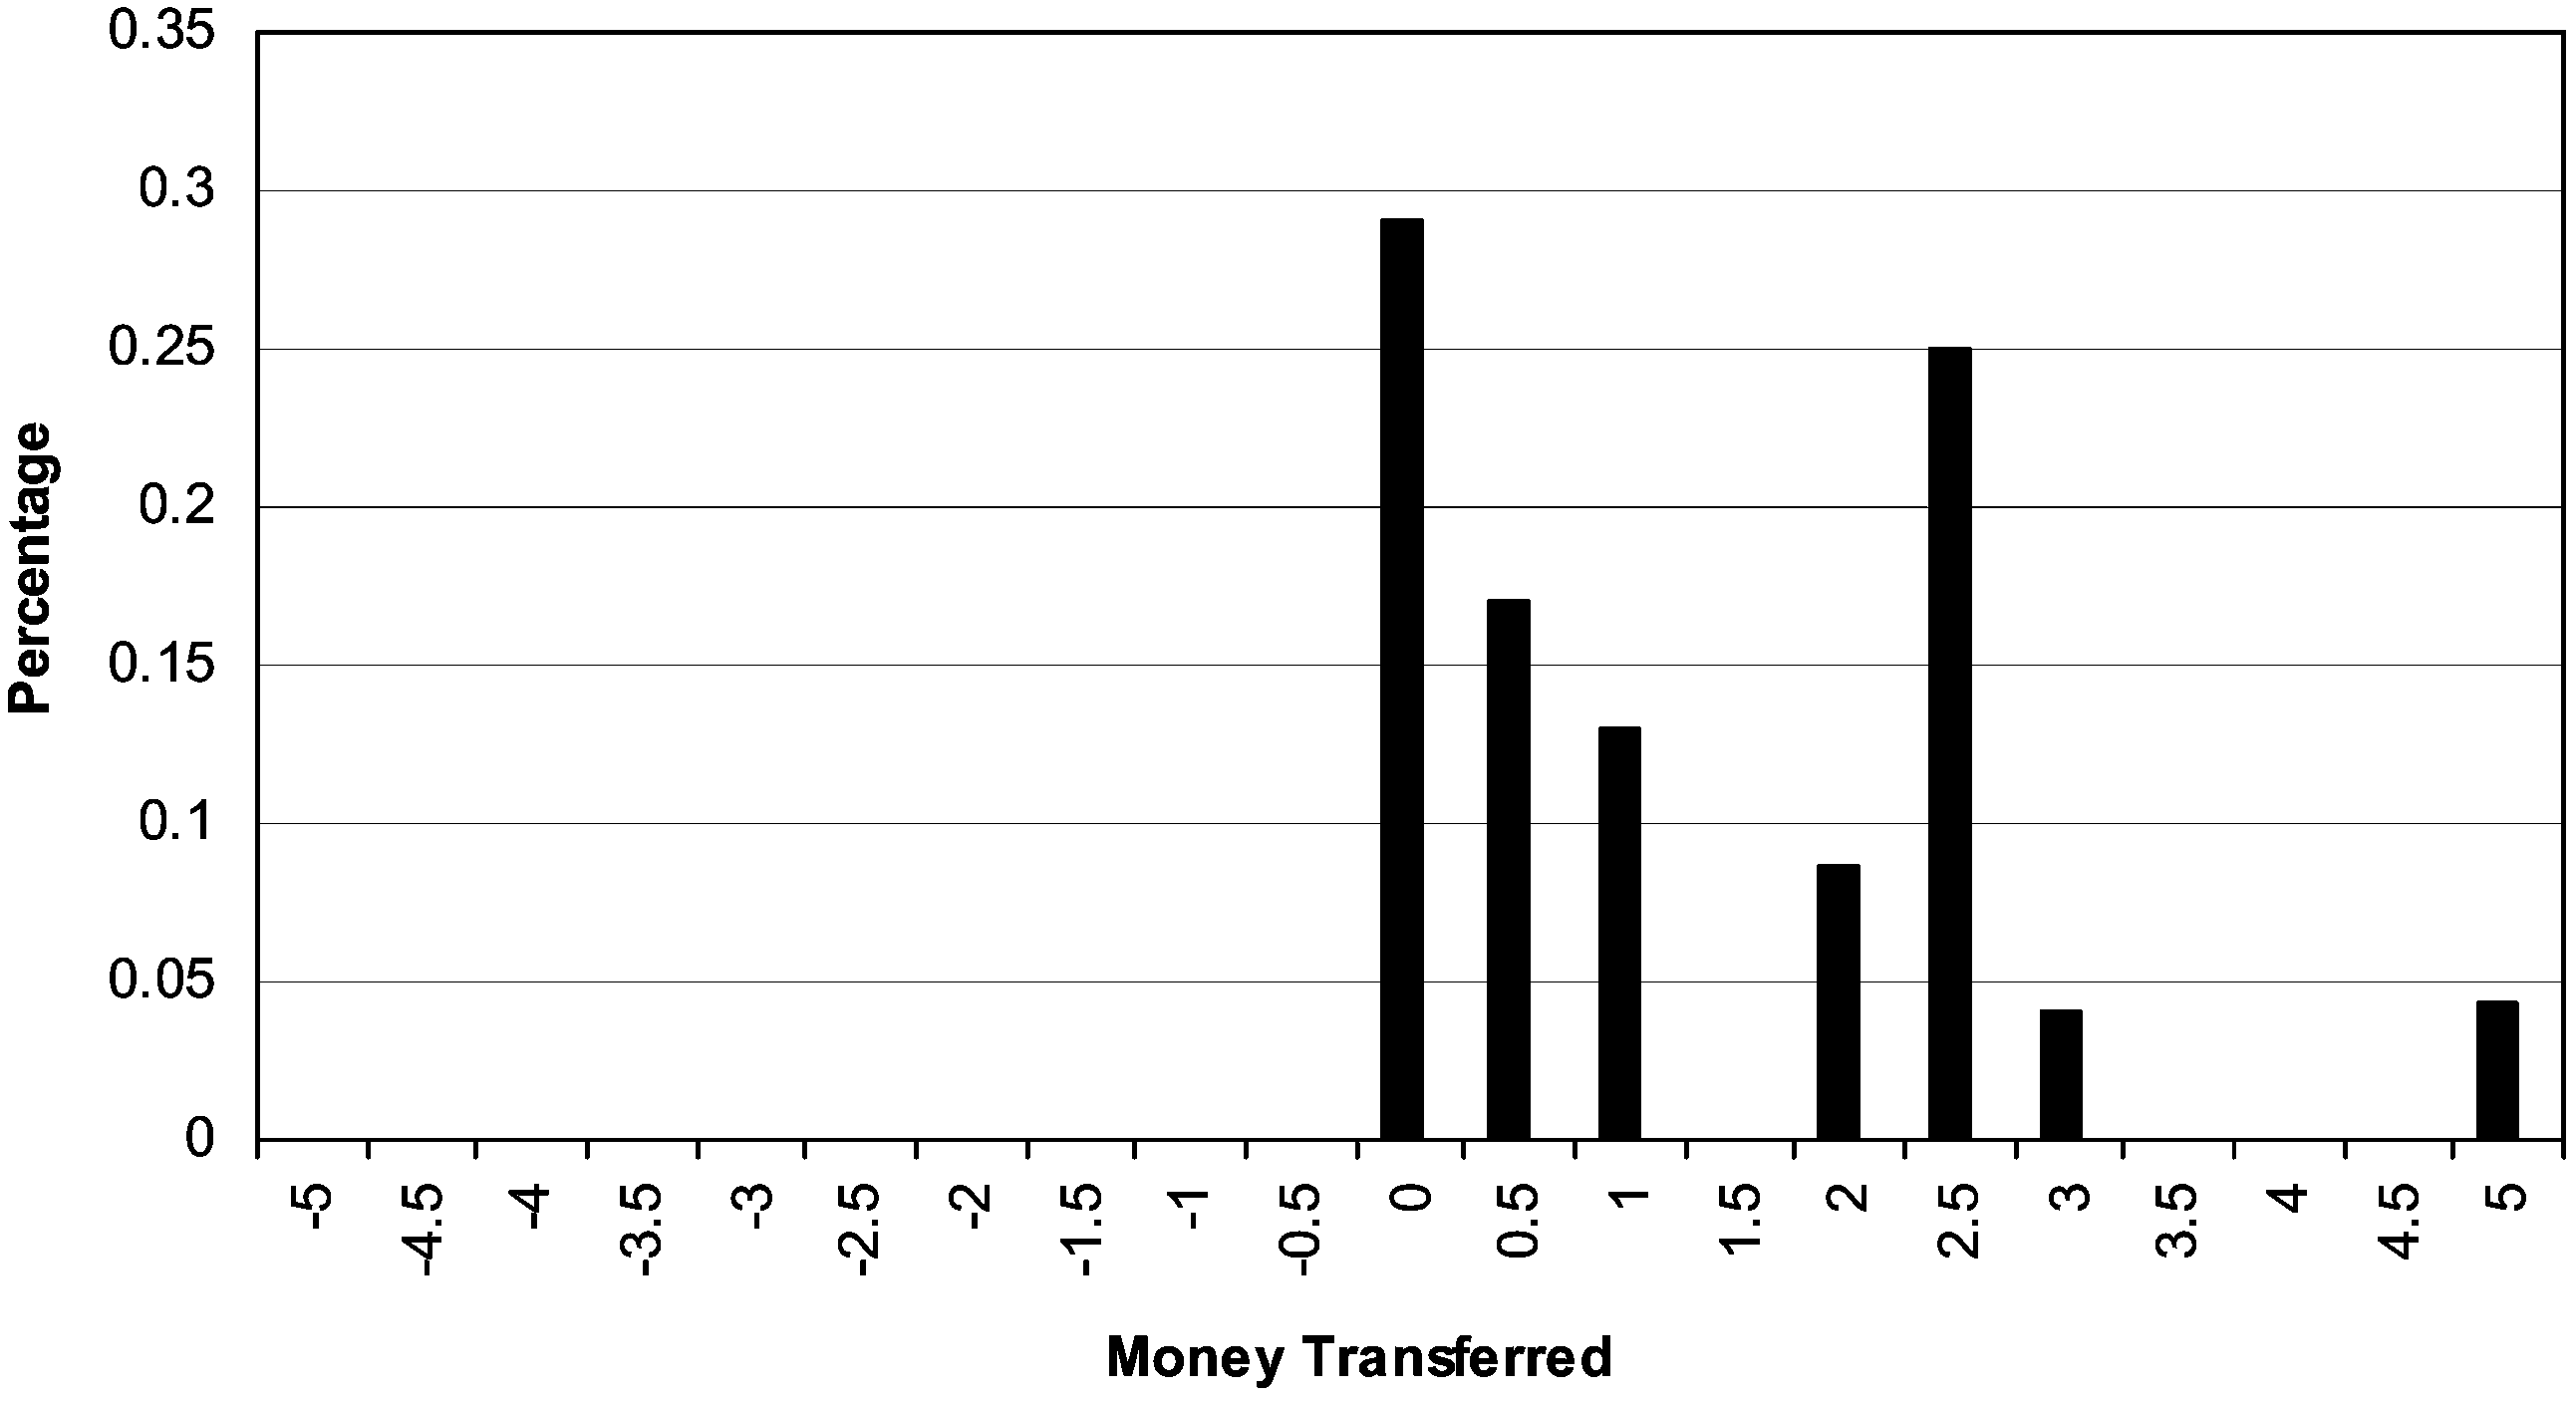
\includegraphics[width=0.4\textwidth]{list1.png}
      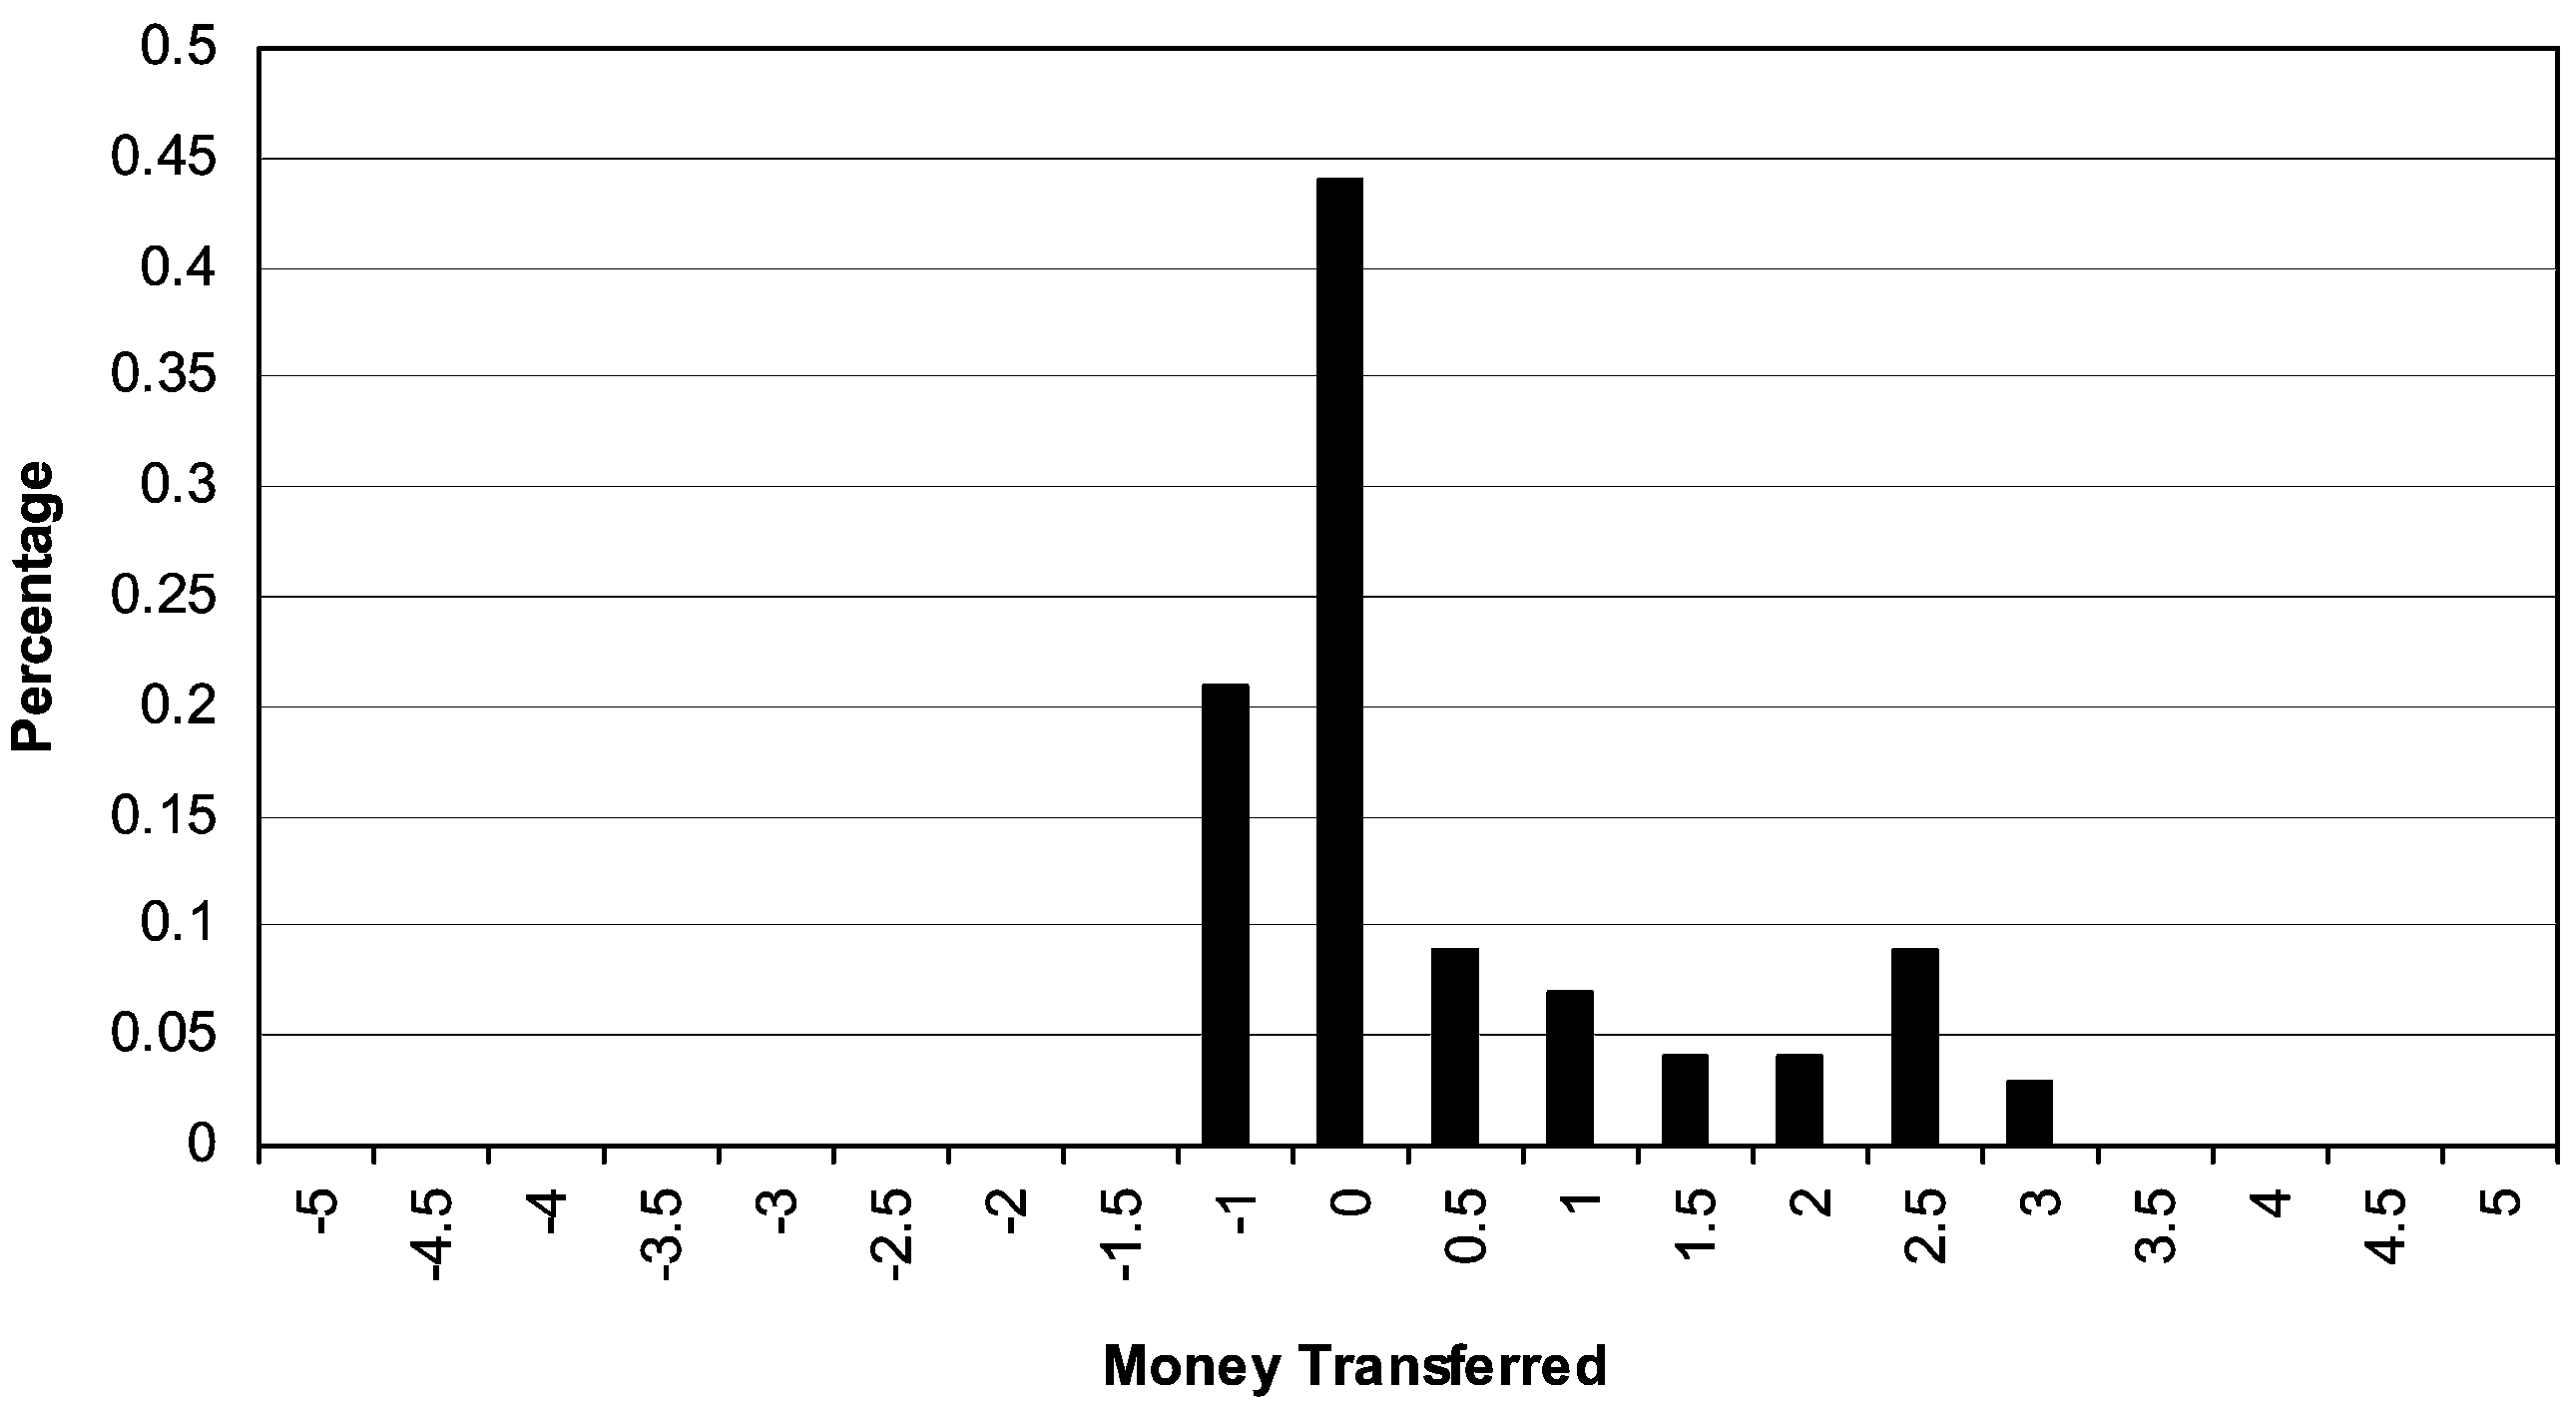
\includegraphics[width=0.4\textwidth]{list2.png}\\
      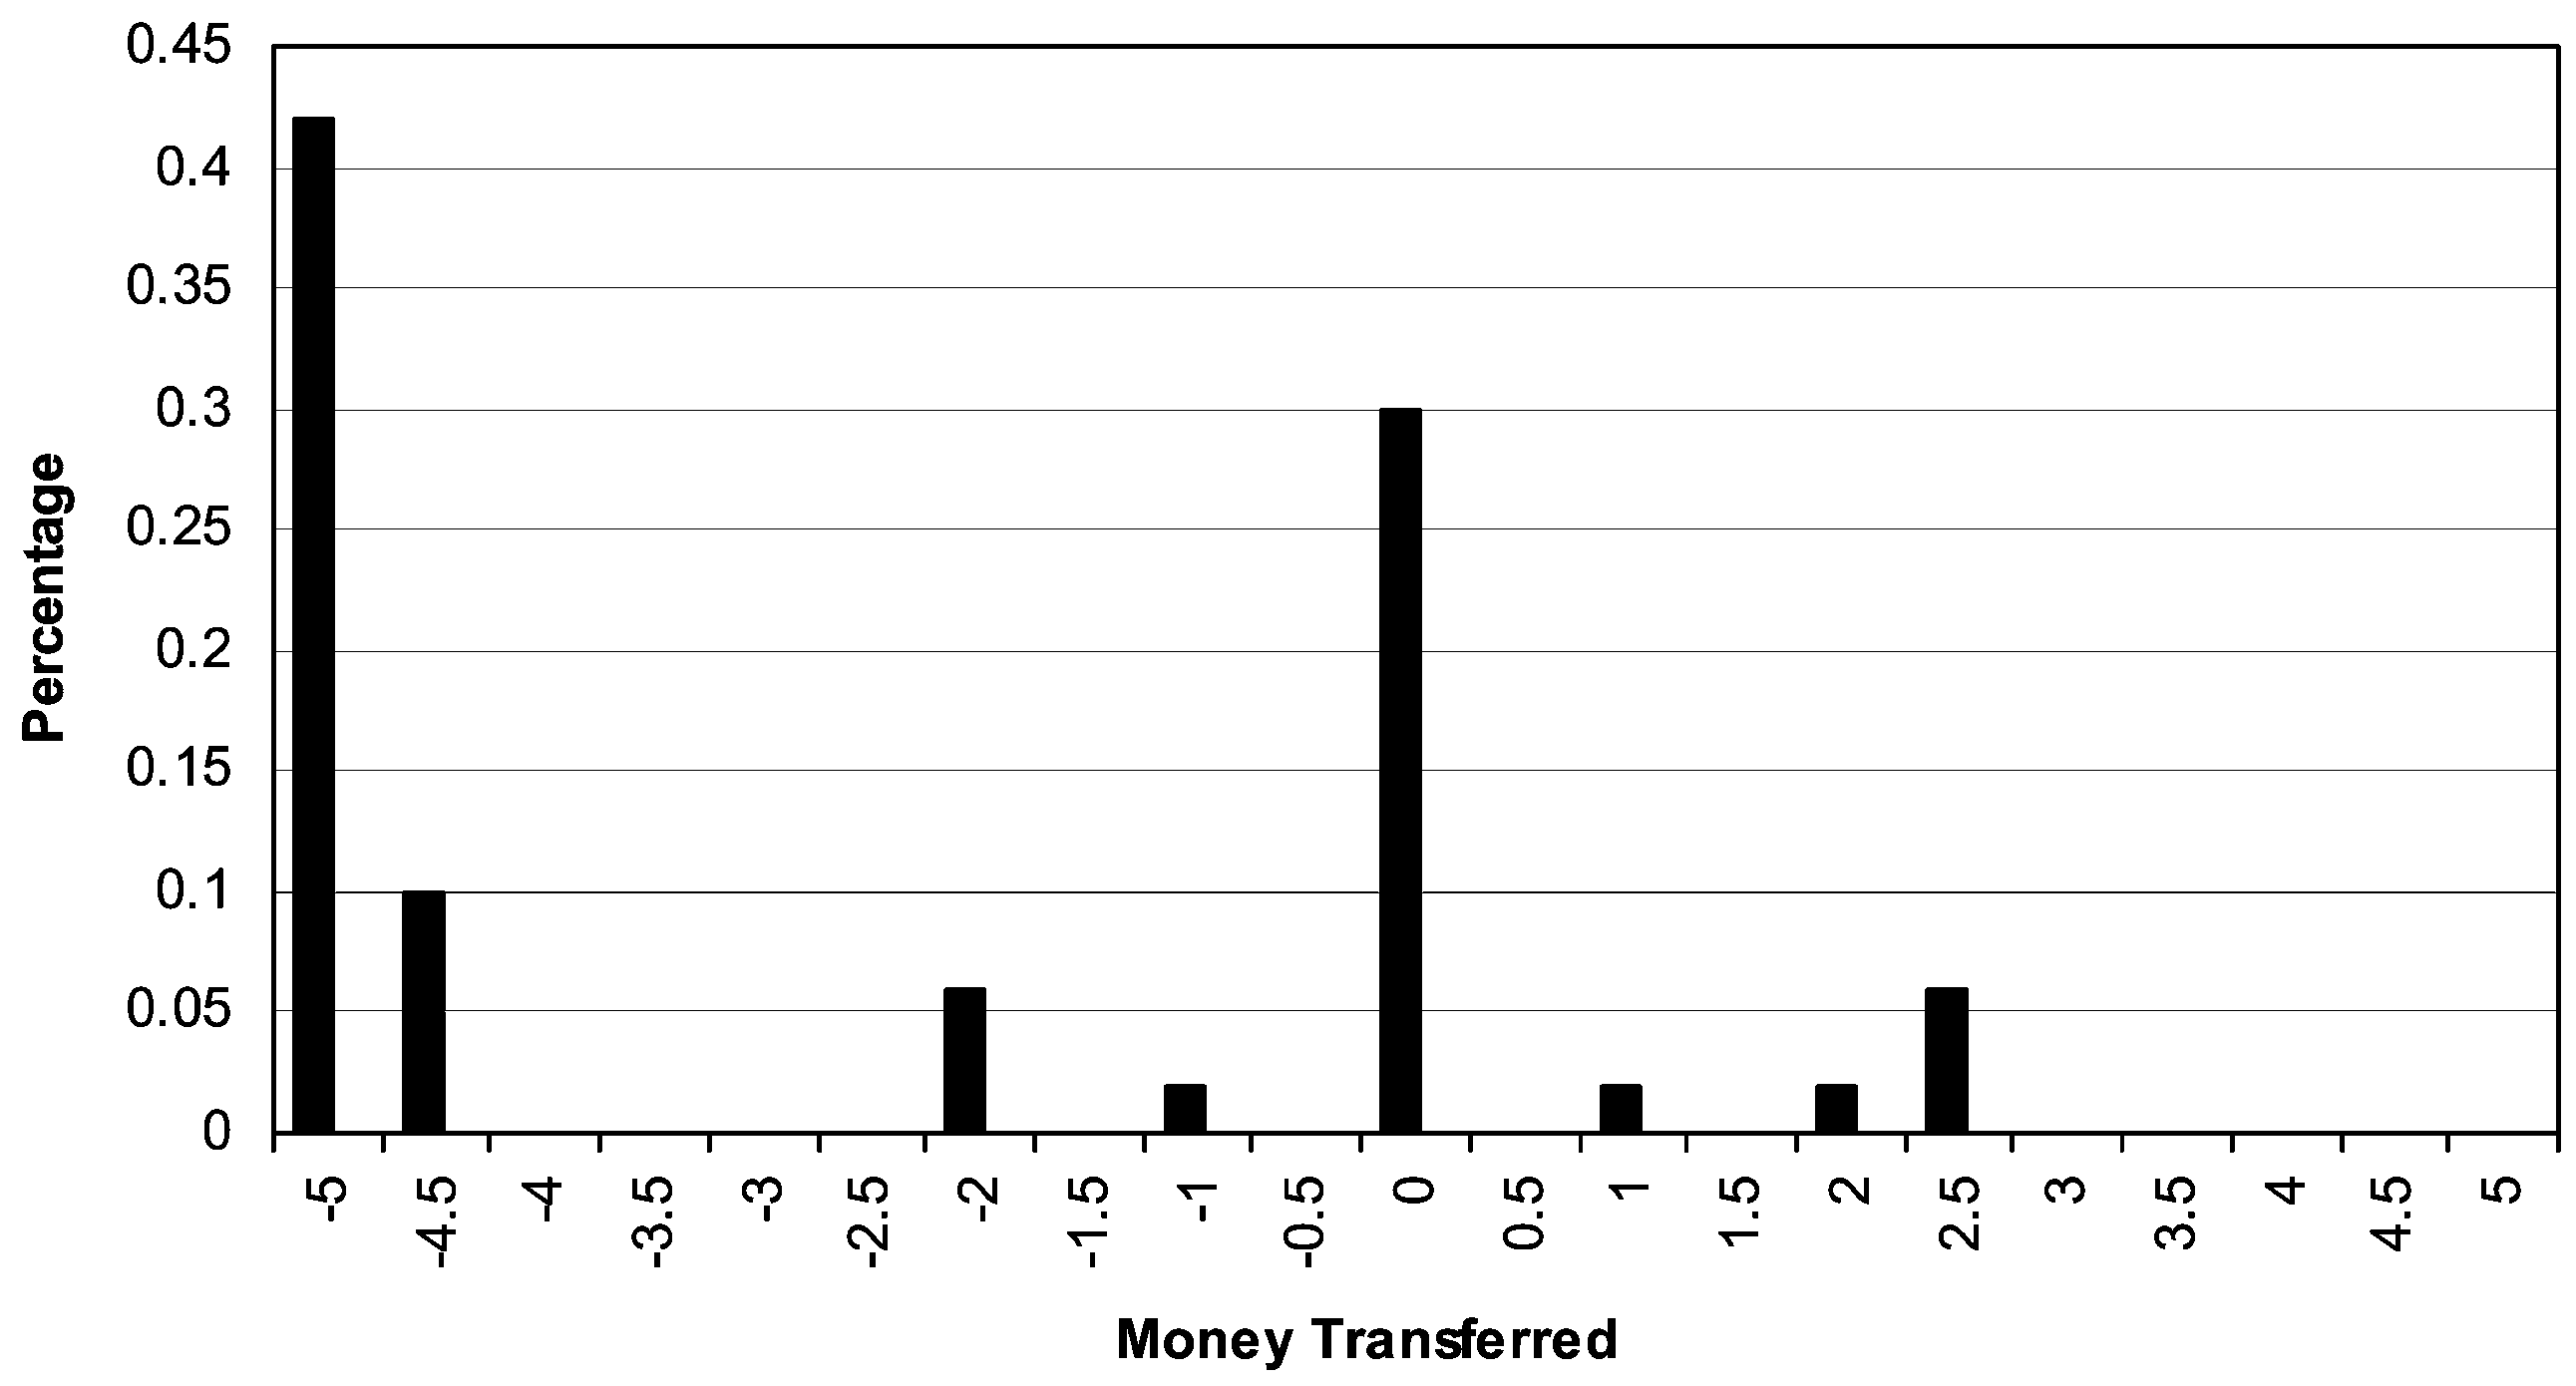
\includegraphics[width=0.4\textwidth]{list3.png}
      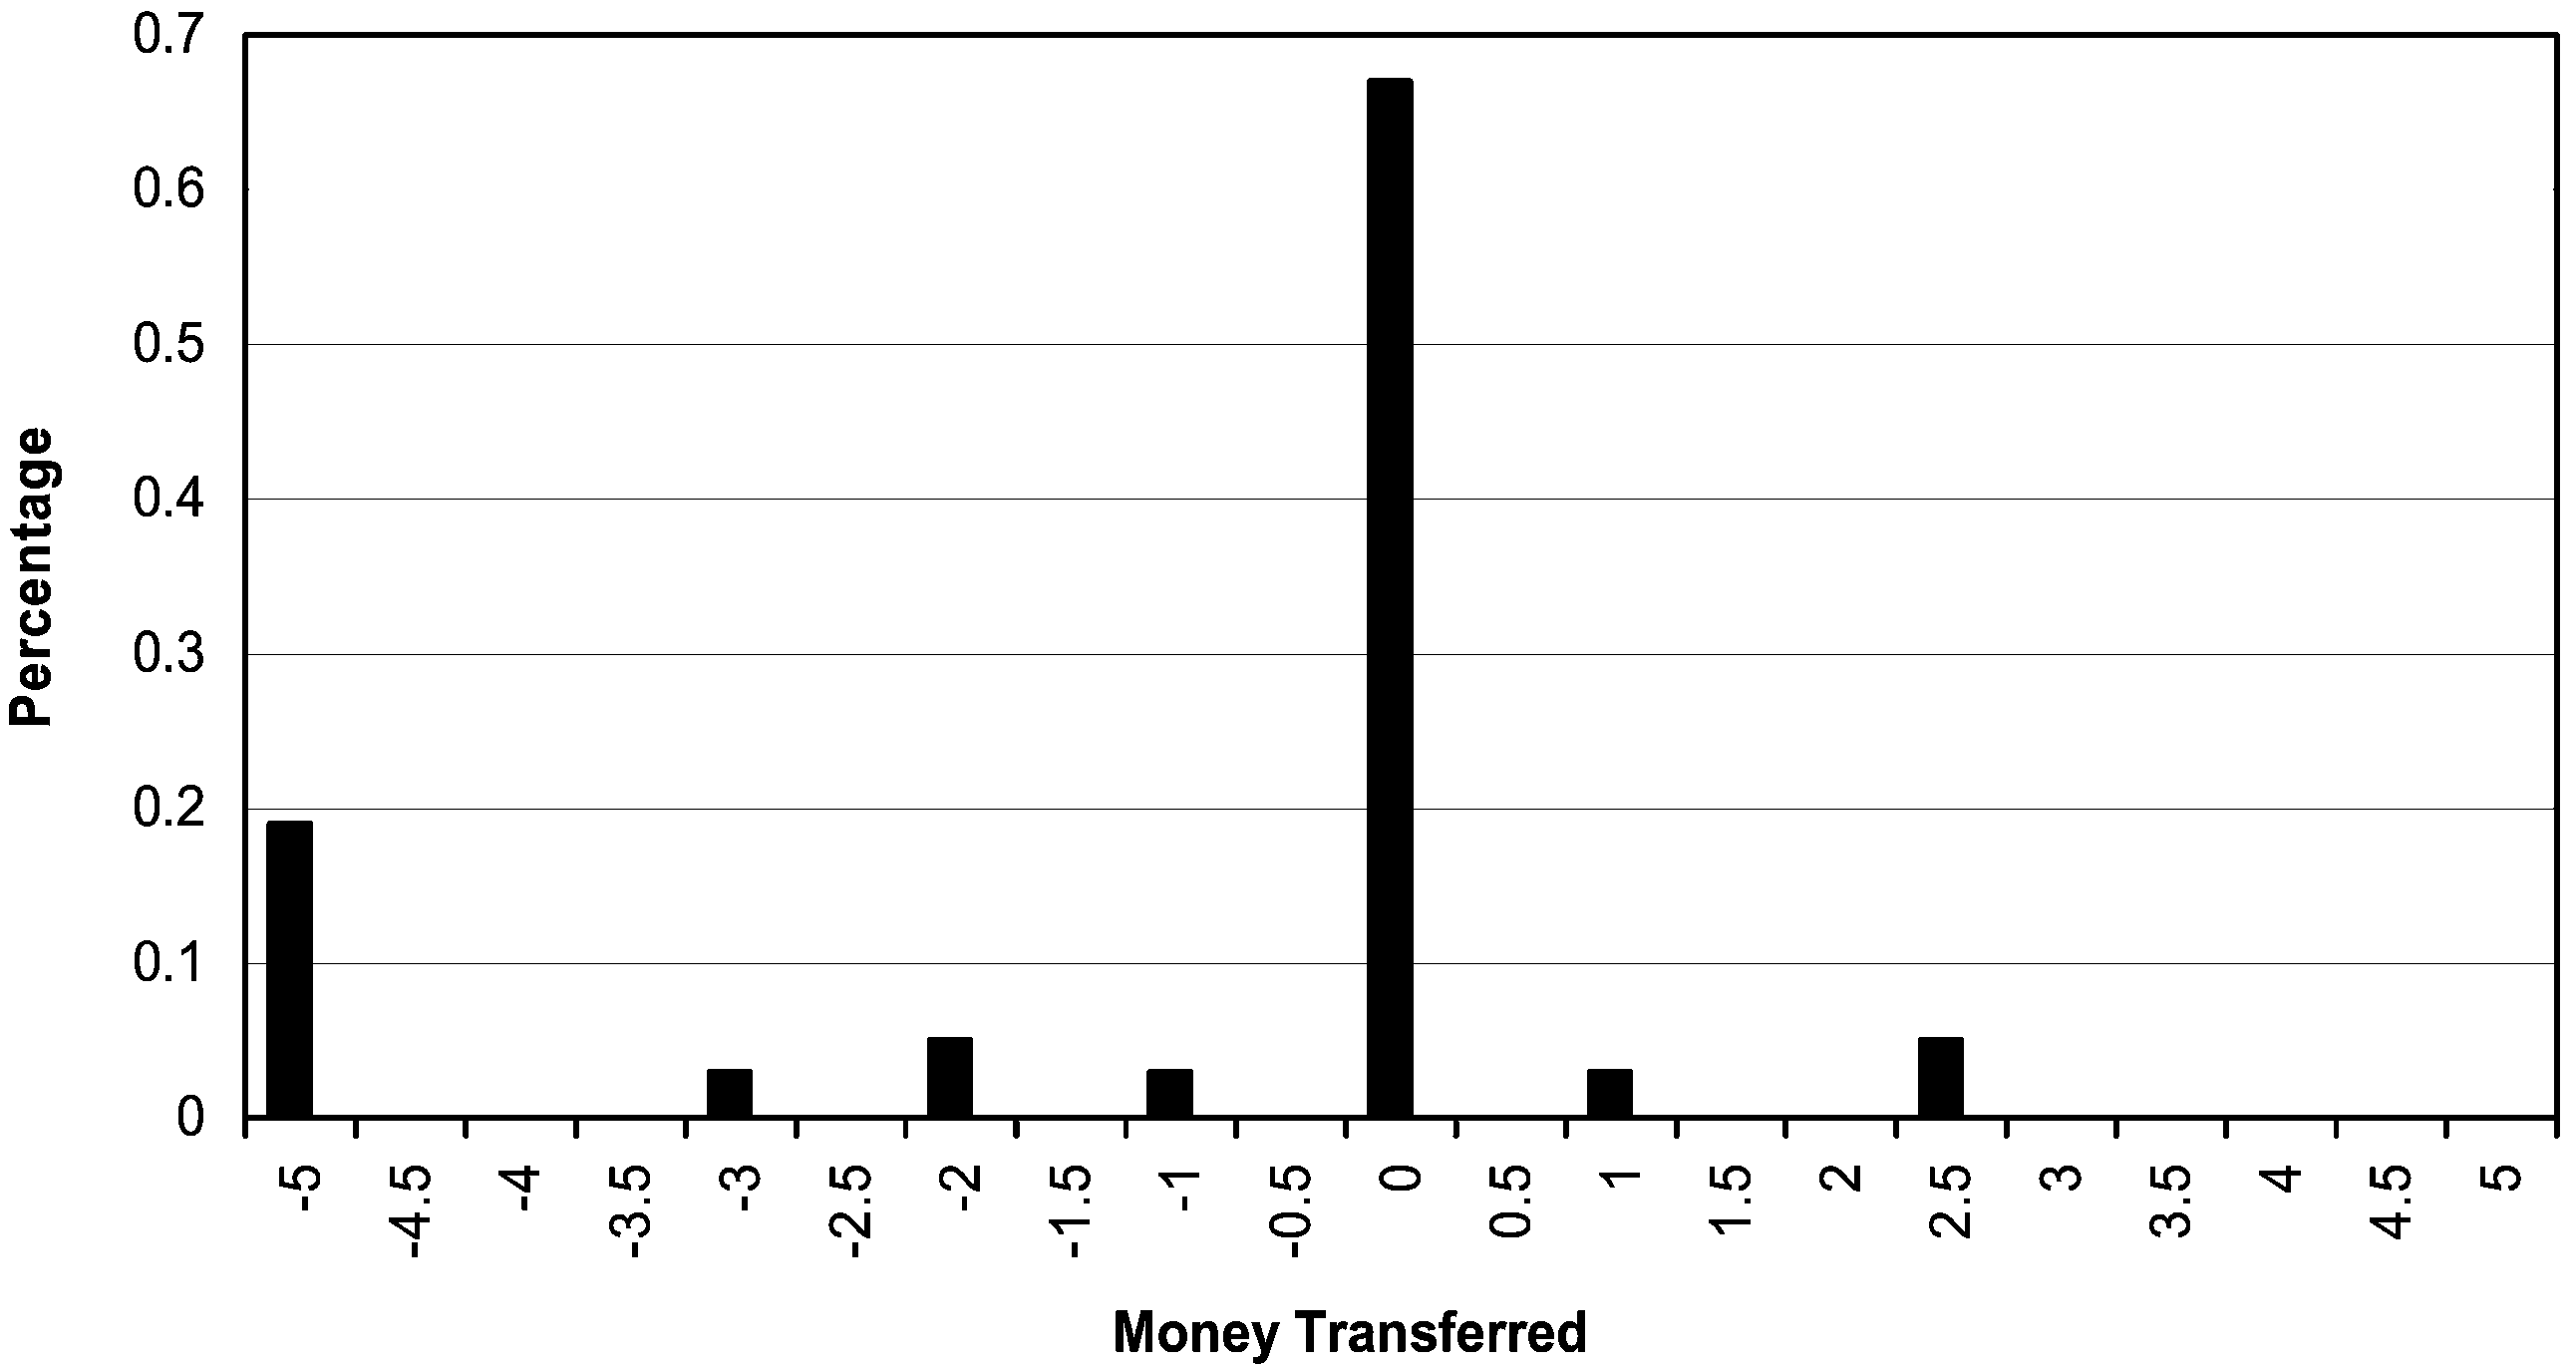
\includegraphics[width=0.4\textwidth]{list4.png}\\
    \subsection{Vyjednávání s ultimátem}
      Tato hra rozšiřuje hru \emph{Diktátor} o druhou fázi, ve které přijemce může buď akceptovat návrh rozdělení
      obdaření, nebo ho odmítnout, což znamená, že nikdo nedostane nic. Poprvé ji uvedl Guth et al. (1982).
      V této hře je příjemci dána nějaká strategická síla k ovlivnění výsledku rozdělení.
      Z předpokladu sobeckosti a použitím subgame-perfect rovnováhy vychází, že navrhovatel nabídne co nejmenší
      možnou částku a příjemce ji akceptuje, protože něco je lepší než nic.

      To se nicméně v laboratoři nepotvrdilo. Typickým výsledkem v rozvinutých zemích je nejčastější
      nabídka 40-50\% obdaření, téměř žádné nabídky nad 50\%, málo nabídek 20-40\%, které jsou v polovině
      případů zamítnuty. Zjevně empirické výsledky neodpovídají teoretickým přepokladům.

      Existuje však vysoká citlivost na detaily provedení:
      \begin{compactitem}
        \item 
          Hoffman et al. (1994): 
          představení hry jako obchodní transakce místo rozdělení daru znamená pokles nejčastějšího návrhu na 40\%.
        \item 
          Pokud jsou role navrhovatele a příjemce rozděleny podle objektivního kritéria výkonu (kvíz, zručnost), 
          klesá nejčastější návrh na 30\%.
        \item
          Bornstein, Yaniv (1998):
          Pokud se rozhodují skupiny po 3-7 lidech je nejčastější návrh 35\% oproti 44\% v případě individuálního
          rozhodování za jinak stejných okolností.
        \item
          Slonim, Roth (1998):
          Čím vyšši je velikost obdaření, tím nižší je procentní návrh a ten je pravděpodobněji akceptován.
          To znamená, že příjemce se rozhoduje spíše podle absolutní hodnoty návrhu. Např. přijme 1\% z \$1000=\$10,
          ale ne 1\% z \$10=\$0.1.

      \end{compactitem}
    \subsection{Dvoukrokové vyjednávání}
      Navrhovatel navrhne částku, příjmece může ihned akceptovat, nebo odmítnout. V tom případě navrhne příjemci,
      ten opět může akceptovat, nebo odmítnout, což by znamenalo, že nikdo nedostane nic.
      Zároveň se uvažuje nižší obdaření v druhém kroku.

      Velikost obdaření v prvním kroku je $X$, v druhém $Y$, $X>Y$. Předpokládejme sobeckost a opět aplikací
      subgame-perfect rovnováhy dostáváme: v druhém kroku příjemce nabídne navrhovateli téměř 0 a navrhovatel přijme.
      Přijemce tedy ví, že v druhém kroku je schopen získat minimálne $Y-\epsilon$, tím pádem odmítne jakýkoukoliv
      nižší nabídku navhrhovatele. Takže nejlepší, co může udělat navrhovatel, je, že nabídne $Y$, příjemce přijme a
      nechá si tak $X-Y$.

      Goeree, Holt (2000) provedli tento experiment a zjistili, zcela opačný výsledek:\\
      \begin{center}
        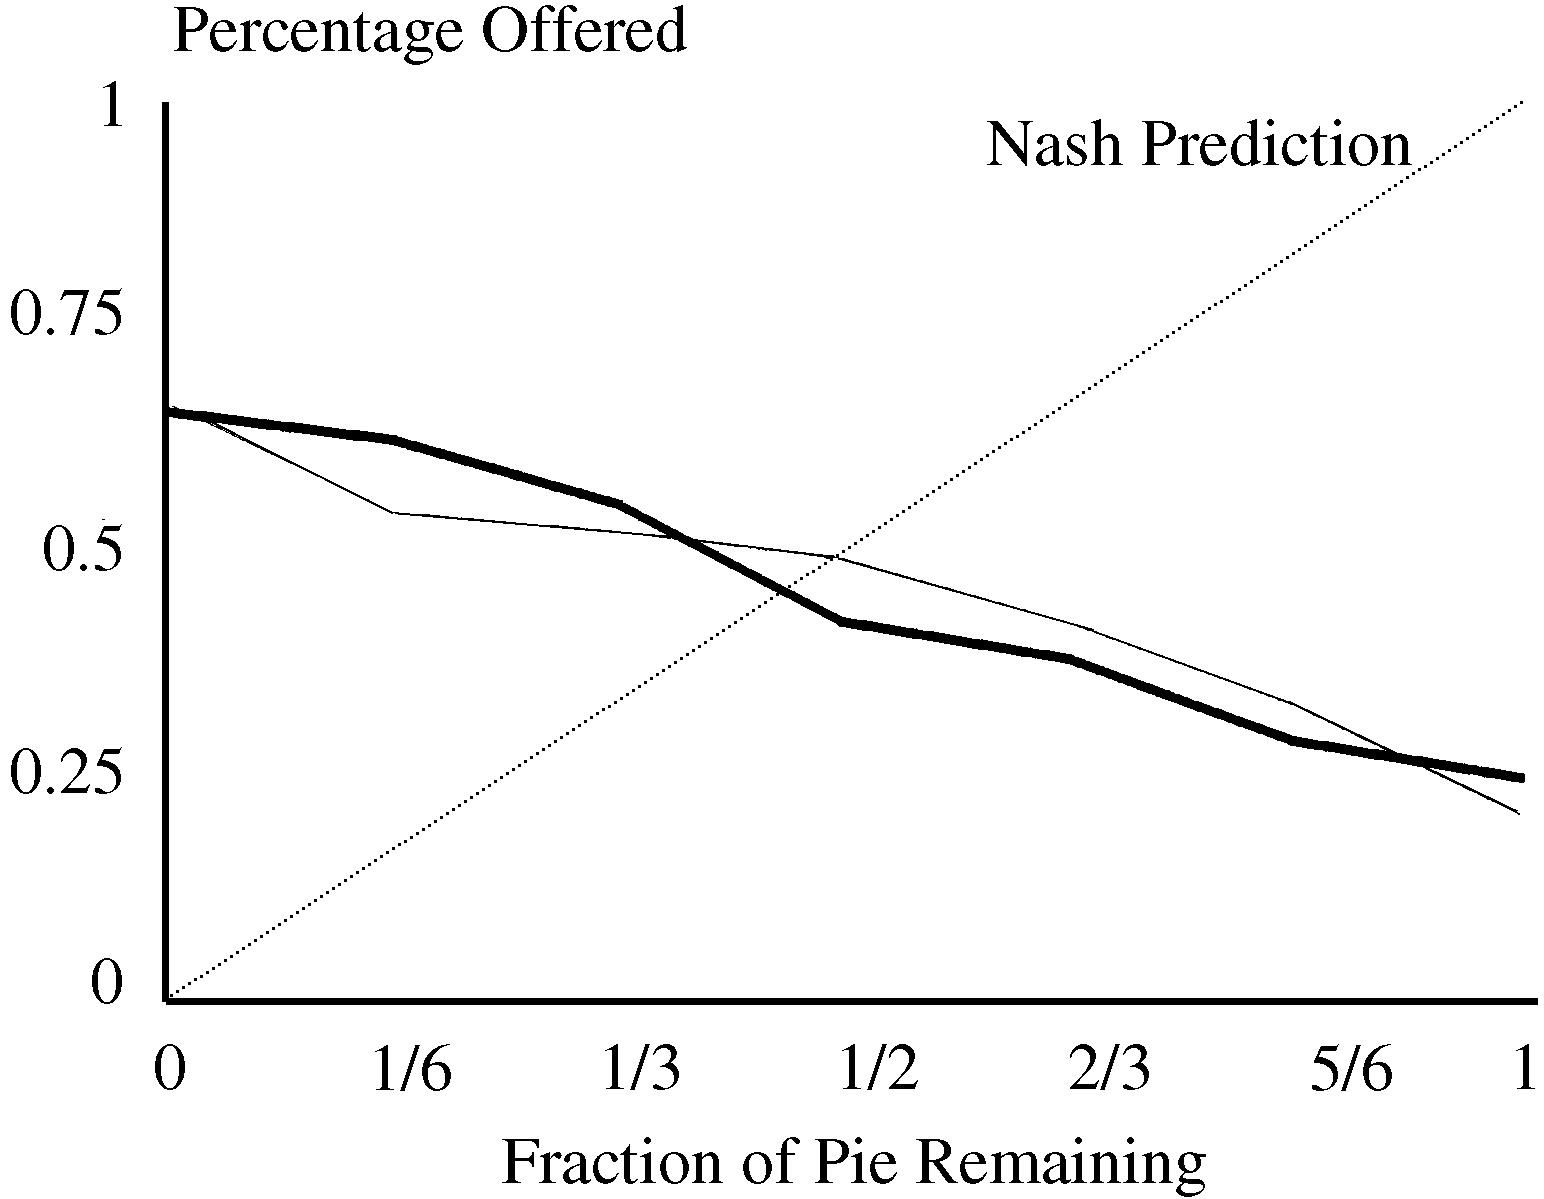
\includegraphics[width=0.7\textwidth]{holt.png}
      \end{center}

    \subsection{Hra investice}
      V této hře jsou dva hráči: investor a makléř. Investor na začátku dostane obdaření $X$ a může část $Y\leq X$
      odeslat makléři. Peníze jsou u makléře zhodnoceny vynásobením koeficientem $\alpha$. Makléř může investorovi
      zpět vrátit $Z\leq\alpha Y$. To si lze představit tak, že makléř pošle zpět zisk snížený o poplatek, nebo
      jednoduše vše ukradne. Celkový výdělek investora je $X-Y+Z$, makléře $\alpha Y-Z$.

      Za předpokladu sobeckosti a aplikací subgame-perfect rovnováhy zjistíme, že makléř nepošle nic zpátky. Investor
      s tím počítá, takže nic nepošle makléři. Není tedy vytvořen žádný ekonomický přebytek. Maximálního přebytku lze
      dosáhnout pokud investor pošle vše. Z tohoto pohledu už rozhodnutí makléře nic neovlivní.

      Berg et el. (1995) provedli tento experiment s parametry $X=\$10$, $\alpha=3$. Jedním z výsledků je tento graf:

      \begin{center}
        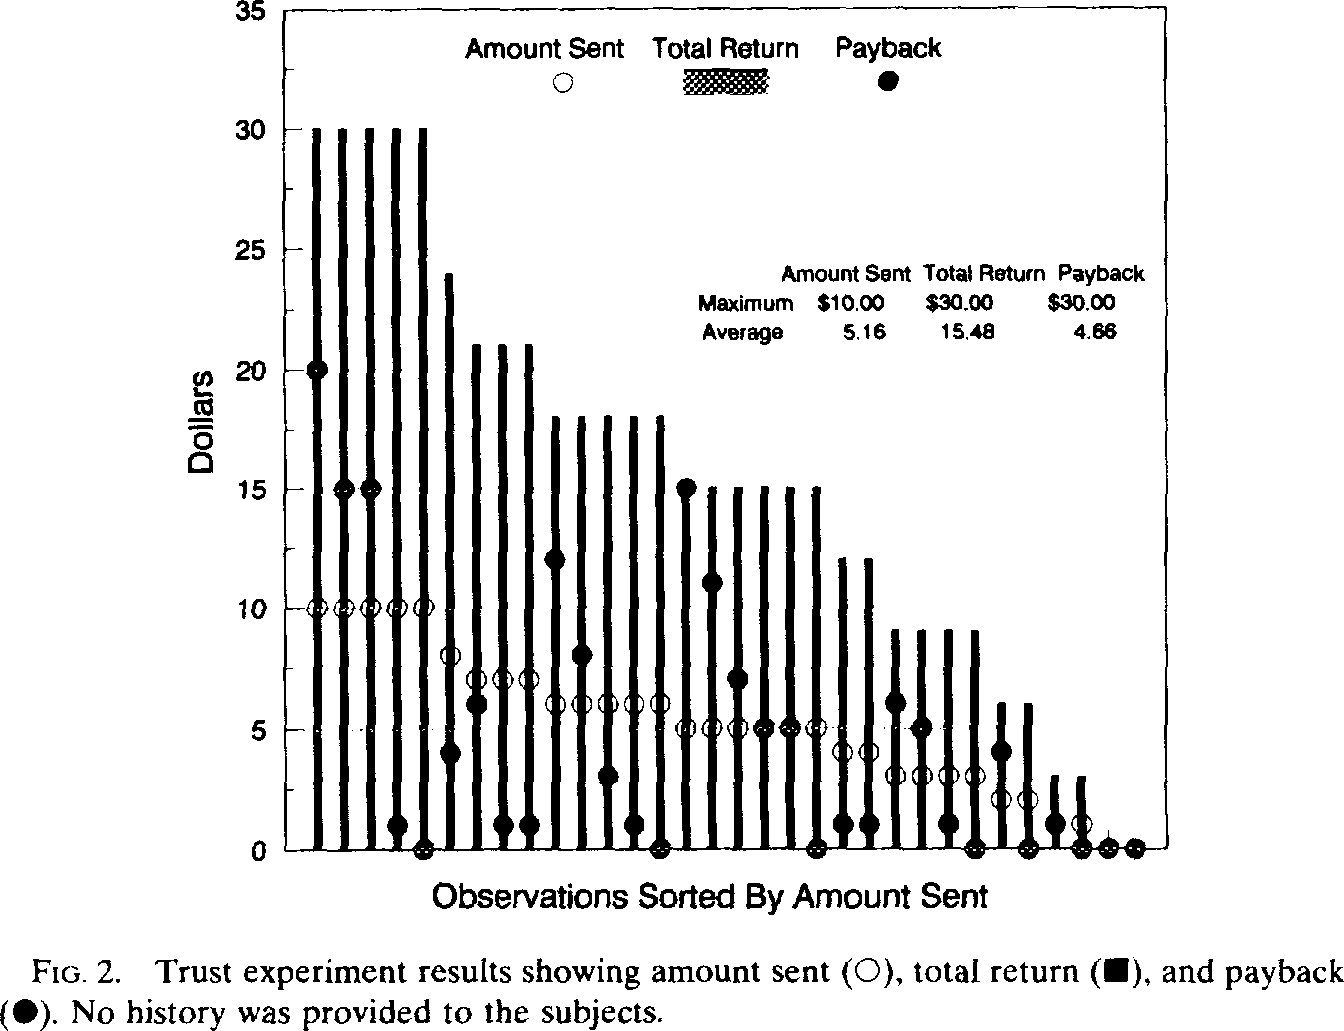
\includegraphics[width=0.6\textwidth]{berg.png}
      \end{center}
      
\clearpage
\begin{thebibliography}{9}
    \bibitem{}
    K. J. Arrow, M. D. Intriligator, Handbook of Mathematical Economics, Vol. 1, ISBN: 0444861262
    \bibitem{} 
    Wikipedia: Imputation (game theory), Cooperative game, Core (game theory), Transferable utility
    \bibitem{}
    L. Pol\'ak: Teorie her, u\v{c}ebn\'y text predmetu Teorie her, Masarykova univerzita
    \bibitem{}
    M. Maschler and B. Peleg, Pacific J. Math. Volume 18, Number 2 (1966), 289-328.
    \bibitem{}
    J. Nash, "Equilibrium points in n-person games", Proceedings of the National Academy of Sciences 36(1), (1950), 48-49.
    \bibitem{}
    Experimental Economics, lecture notes, Peter Katuščák, M.A., M.B.A., Ph.D.
    \bibitem{}
    Robert Forsythe, Joel L. Horowitz, N.E. Savin, Martin Sefton, Fairness in Simple Bargaining Experiments, Games and Economic Behavior, Volume 6, Issue 3, May 1994, Pages 347-369, ISSN 0899-8256, 10.1006/game.1994.1021.
(http://www.sciencedirect.com/science/article/pii/S0899825684710219)
    \bibitem{}
    Hardnose the Dictator,
Todd L. Cherry, Peter Frykblom and Jason F. Shogren,
The American Economic Review,
Vol. 92, No. 4 (Sep., 2002), pp. 1218-1221
    \bibitem{}
    List, John A., On the Interpretation of Giving in Dictator Games. Journal of Political Economy, Vol. 115, No. 3, 2007. Available at SSRN: http://ssrn.com/abstract=1076569
    \bibitem{}
    Werner Güth, Rolf Schmittberger, Bernd Schwarze, An experimental analysis of ultimatum bargaining, Journal of Economic Behavior \& Organization, Volume 3, Issue 4, December 1982, Pages 367-388, ISSN 0167-2681, 10.1016/0167-2681(82)90011-7.
(http://www.sciencedirect.com/science/article/pii/0167268182900117)
    \bibitem{}
    Learning in High Stakes Ultimatum Games: An Experiment in the Slovak Republic,
Robert Slonim and Alvin E. Roth,
Econometrica,
Vol. 66, No. 3 (May, 1998), pp. 569-596
    \bibitem{}
    Jacob K. Goeree, Charles A. Holt, Asymmetric inequality aversion and noisy behavior in alternating-offer bargaining games, European Economic Review, Volume 44, Issues 4-6, May 2000, Pages 1079-1089, ISSN 0014-2921, 10.1016/S0014-2921(99)00048-3.
(http://www.sciencedirect.com/science/article/pii/S0014292199000483)
    \bibitem{}
    Joyce Berg, John Dickhaut, Kevin McCabe, Trust, Reciprocity, and Social History, Games and Economic Behavior, Volume 10, Issue 1, July 1995, Pages 122-142, ISSN 0899-8256, 10.1006/game.1995.1027.
(http://www.sciencedirect.com/science/article/pii/S0899825685710275)
\end{thebibliography}
\end{document}
